% =========================================================
% INTRODUCCIÓN A LA CRIMINOLOGÍA AMBIENTAL
% =========================================================
El crimen se define como un evento complejo que ocurre cuando cuatro cosas coinciden: la ley, un agresor, una víctima y un lugar. La "criminología ambiental" se pregunta cómo es que esta cuarta dimensión del crimen interactúa con las otras tres dimensiones para producir un evento criminal\cite{brantingham1981}. Por tanto, para conseguir un análisis completo del crimen, es necesario contemplar estas cuatro dimensiones bajo el contexto específico de la zona que se desea investigar.

Hasta antes de la década de 1990, la mayor parte de los intentos por explicar los eventos criminales se basaban en modelos criminológicos unicausales, centrados principalmente en las características del delincuente. Sin embargo, a partir de la década de 1970 surgió una línea de pensamiento que proponía un análisis enfocado específicamente en el \textit{evento criminal} como unidad de estudio, reconociendo la necesidad de explicarlo como resultado de "complejos patrones etiológicos de comportamiento"\cite{brantingham1993}.

% =========================================================
% NIVELES DE ANÁLISIS
% =========================================================
\subsection{Los niveles de análisis}
La escala es muy importante en el análisis espacial de un crimen. No es lo mismo investigar la concentración de crímenes a nivel República mexicana, que a nivel unidad habitacional. Así, los niveles de análisis refieren a esta escala en que se estudia la repercusión de la cuarta dimensión del crimen(el lugar) y actualmente se dividen en tres niveles separados: Macro-análisis, meso-análisis y micro-análisis.

\textit{El macro-análisis} envuelve los estudios al nivel más alto de agregación espacial. Involucra comúnmente estudios de la distribución de crímenes entre países, entre estados o provincias. \textit{El meso-análisis} envuelve estudios en un nivel intermedio. Su estudio involucra el análisis del crimen en subáreas de una ciudad o una metrópolis. Finalmente, \textit{el micro-análisis} involucra el estudio de lugares específicos donde sucede el crimen. Se enfoca en el tipo de edificios y su posicionamiento\cite{brantingham1981}.

El nivel de análisis es de suma importancia ya que los patrones del crimen varían dependiendo del nivel seleccionado. La homogeneidad es un artefacto de la escala del análisis según nos dice Brantingham en su estudio sobre robo en 1970 basado en datos de diferentes escalas. En cada caso, se concluye que una unidad aparentemente homogénea en un nivel de análisis puede desglosarse en subunidades que tienen tasas de criminalidad muy diferentes\cite{brantingham1976}.


% =========================================================
% ELECCIÓN DE VARIABLES / CRÍTICAS A DEFENSIBLE SPACE
% =========================================================
\subsection{La importancia de la elección de variables}
Si bien elegir el nivel correcto es parte importante del análisis del crimen no es suficiente pues es necesario considerar que una misma variable funciona mejor en un nivel específico de análisis que en otro. Si bien las ideas de Oscar Newman en "Defensible Space: Crime Prevention through Urban Design (1972)" fueron revolucionarias y atrajeron el interés de muchos criminólogos, urbanistas, geógrafos, psicólogos ambientales y arquitectos\cite{brantingham1981}, es cierto que ha sido objeto de muchas críticas metodológicas que resultan relevantes para el diseño de un modelo de crimen verdaderamente funcional.

Newman propuso que a través de la manipulación de las configuraciones espaciales y de construcción, se pueden crear áreas por las cuales la gente se preocupará\cite[p.~206]{OscarNewman1973}. Sin embargo, Mayhew (1979, 1981) concluyó que algunas características de diseño a nivel meso son mucho más criticas que las propuestas por Oscar Newman en un nivel micro\cite{brantingham1981}. En la misma línea, Merry (1981) encontró que las personas no vigilan automáticamente su entorno incluso cuando el diseño físico lo permite, y que los delincuentes son conscientes de ello\cite{merry1981}. Estas críticas sugieren que el nivel de resolución espacial y el tipo de variable analizada son decisiones metodológicas independientes: una resolución fina (a nivel de manzana o segmento de calle) permite capturar la heterogeneidad real del fenómeno delictivo, pero no garantiza que las variables elegidas en ese nivel tengan poder explicativo suficiente.

Esto es un claro ejemplo de las dimensiones del análisis y fundamenta la idea de que un análisis completo del crimen necesita tomar la totalidad de éstas en cuenta\cite{brantingham1981}. Por esta razón, la elección de variables para un modelo de criminología ambiental requiere un análisis profundo sobre el factor social detrás de ellas y de ser posible, fundamentos sobre la utilidad que tienen esas variables en el estudio del crimen.


% =========================================================
% TEORÍA DE LOS PATRONES DELICTIVOS
% =========================================================
\subsection{Teoría de los patrones delictivos}
Con la nueva corriente de pensamiento que surgió en la década de 1970 y el trabajo complementario que provocó, se propone mirar al crimen como un evento complejo. Sin embargo, inclusive en este nivel de complejidad es posible discernir una serie de patrones aplicables tanto a criminales como al crimen en sí. \cite[p.~266]{brantingham1993}. La teoría se deriva de los acercamientos multidisciplinarios para entender el crimen y la criminalidad a partir de la teoría de la elección racional, la teoría de las actividades rutinarias, la criminología ambiental, el análisis estratégico, la teoría del estilo de vida, la prevención del crimen a través del diseño ambiental, la prevención del crimen situacional, el análisis de puntos calientes y la teoría de oportunidades\cite[p.~284]{brantingham1993}.

\subsubsection{Teoría de la elección racional}
Propuesta por Cornish y Clarke en 1986, propone una metodología de toma de decisiones para explicar el crimen. Establece que los agresores buscan obtener un beneficio propio al realizar actos delictivos, lo cual los lleva a tomar ciertas decisiones. De igual manera, estos actos delictivos muestran una especie de ``racionalidad'', que suele estar limitada por el tiempo, la habilidad y la disponibilidad de información\cite{cornish1986}.

Segundo, para evaluar estos comportamientos se adoptó un enfoque centrado en el ``crimen'' más que en el agresor en sí. Este enfoque permite apreciar de mejor manera las distinciones que existen en la toma de decisiones según cada tipo de ofensa. Por último, plantea una distinción clara entre la \textit{implicación criminal}, que es el proceso por el cual alguien se involucra, continúa y desiste del crimen, y el \textit{evento criminal} propiamente dicho, que se refiere al cometimiento de un delito específico\cite{cornish1986}.

Esta distinción es central para la teoría: dado que la implicación criminal y el evento criminal responden a variables distintas y se desarrollan en escalas temporales diferentes, requieren modelos de decisión separados. Así, la teoría de la elección racional adopta un enfoque situacional para explicar el evento delictivo específico, mientras reconoce que la disposición a delinquir a largo plazo depende de procesos de aprendizaje e incentivos acumulados a lo largo de la carrera criminal.

\subsubsection{Teoría de las actividades rutinarias}
Propuesta por Cohen y Felson en 1979. En esta teoría desecha el enfoque en el agresor y se centra en el hecho criminológico. Establece que la mayoría de los actos delictivos requieren la convergencia, en el espacio y en el tiempo, de delincuentes potenciales, objetivos adecuados y la ausencia de guardianes capaces contra el crimen. La falta de cualquiera de estos tres elementos es suficiente para prevenir la aparición de un delito predatorio de contacto directo realizado con éxito.\cite{cohenfelson1979}.

En general, este enfoque tiene su origen en la teoría de la ecología humana de la estructura de las comunidades de Amos Hawley (1950), la cual confiere al ambiente físico una importancia fundamental en la actividad del individuo\cite{canopanos2018}.

Se definen a las actividades rutinarias como aquellas actividades recurrentes y prevalentes que cubren las necesidades básicas tanto de la población como de los individuos\cite{cohenfelson1979}. Dentro de estas actividades entran aquellas como el trabajo, lugares de privisión de alimento, ocio y de interacción social. 

De este modo, los autores establecen que la propia estructura social produce una convergencia de los factores mencionados y que, la dispersión de actividades lejos del hogar y de la familia pueden incrementar las posibilidades del delito\cite{cohenfelson1979}. De esta manera, el factor "oportunidad" sería un elemento clave en la explicación del delito\cite{canopanos2018}.

\subsubsection{Teoría del estilo de vida}
También se le llama teoría de la victimización personal. Fue desarrollada por Hindelang, Gottfredson y Garofalo en 1978. Establece que que un individuo sufra una victimización depende profundamente del "Estilo de vida"\cite{hindelang1978}. Este estilo de vida se define básicamente como aquellas actividades rutinarias del día a día.

A diferencia de los trabajos mencionados, se enfoca profundamente en la dimensión de la victima. Su modelo básico propone que la estructura social y las expectativas definen restricciones a las que los individuos deben adaptarse para funcionar en la sociedad\cite{hindelang1978}. Estas restricciones crean una adaptación que se ve reflejada en un estilo de vida que en mayor o menor medida expondrán a los individuos a la victimización. La figura \ref{fig:estilo_de_vida_modelo} muestra el modelo propuesto por los autores.

\begin{figure}
    \centering
    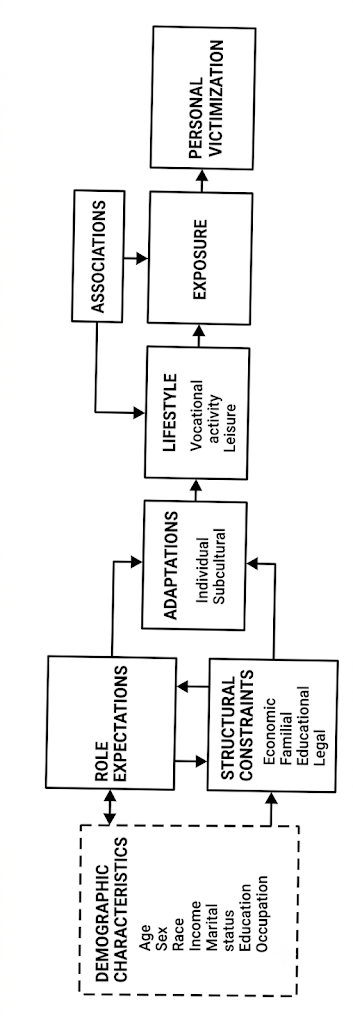
\includegraphics[width=0.5\linewidth]{figures/capitulo3_marco_teorico/3.1_criminologia_ambiental/personal_victimization_model.png}
    \caption{Modelo de la victimización personal.}
    \label{fig:estilo_de_vida_modelo}
    \footnotesize{Nota: Adaptación propia con base en la Figura 11-1 de \cite[p.~243]{hindelang1978}.}
\end{figure}

\subsubsection{Prevención del crimen a través del diseño ambiental}
Acuñada por C. Ray Jeffrey en 1971 en su libro del mismo nombre. En él, argumentó que la modificación de características específicas del diseño urbano reduciría la criminalidad\cite{brantingham1981}. Jeffrey principalmente, establece que\cite{jeffery1971}:

\begin{enumerate}
    \item El crimen puede ser controlado mediante el diseño urbano. Las ciudades son inseguras porque presentan oportunidades para la realización de actos delictivos.
    \item Las ciudades también pueden diseñarse de manera que aumenten el contacto humano, aunque sea de naturaleza íntima. La anomia, la soledad y la alienación no necesariamente caracterizan la vida urbana.
    \item La renovación urbana puede sustituir al sistema de bienestar y se puede poner a las personas a trabajar para construir un entorno que apoye el desarrollo biológico y social de sus habitantes.
\end{enumerate}

\subsubsection{Prevención del crimen situacional}
La prevención del crimen situacional fue propuesta en 1980 por Ronald V. Clarke. Ésta comprende las medidas de reducción de oportunidad que, están dirigidas a formas específicas de crimen; incluyen la gestión, diseño o manipulación del entorno inmediato en una manera tan sistemática y permanente como sea posible; y que hacen al crimen más difícil y riesgoso, o al menos menos beneficioso y excusable para un amplio rango de infractores\cite{clarke1997}.

Algunas de las características más importantes de la definición que nos pueden ayudar a definir de mejor manera este concepto son las siguientes\cite{clarke1997}:

\begin{itemize}
    \item El crimen situacional debe ser diseñada para categorías altamente específicas del crimen. La necesidad de medidas especializadas hacia agresiones particulares no debe ser interpretado como una implicación de que los agresores son especialistas, sino que ciertos crímenes dependen de la construcción de las oportunidades propias de un entorno.
    \item La prevención del crimen situacional no dibuja distinciones entre criminales y las otras personas. Parte de la premisa que todas las personas tienen algo de probabilidad de cometer un crimen dependiendo de las circunstancias.
    \item Cambiar el entorno está diseñado para afectar las evaluaciones hechas por potenciales agresores acerca del costo y los beneficios asociados con cometer un crimen en particular.
    \item Los juicios hechos por potenciales agresores incluyen alguna evaluación del costo moral de agredir. Muchos podemos estar dispuestos a robar pequeños objetos de nuestros empleadores; sin embargo, muy pocos de nosotros estamos dispuestos a robar a una mujer de la tercera edad. Por esto, la moral define en gran medida el alcance del desplazamiento.
    \item Es deliberadamente general para ser aplicable a cualquier tipo de crimen.
\end{itemize}

Asimismo, la prevención situacional del crimen se compone de cuatro componenetes principales. Primero, una base teórica que se apoya principalmente en los enfoques de actividad rutinaria y elección racional; segundo, una metodología estándar basada en el paradigma de la investigación-acción; tercero, un conjunto de técnicas de reducción de oportunidades y finalmente, un cuerpo de prácticas evaluadas que incluye estudios de desplazamiento\cite{clarke1997}.

\subsubsection{Análisis de puntos calientes}
Propuesto por Lawrence Sherman, Patrick Gartin y Michael Buerger en 1989. El artículo busca entender la repetición de la victimización enfocándose en las locaciones individuales como unidad de análisis. En él, los autores establecen que el crimen se concentra de gran manera en solo una serie de ``puntos calientes'' de crimen \cite{sherman1989}. De esta manera, no solo el crimen es más frecuente en algunas ``zonas'' específicas, sino que también el estudio de estas zonas a un nivel micro puede revelar datos mucho más prácticos para la prevención del crimen que el enfoque en áreas más extensas.

El artículo analiza las llamadas de servicio policial en Minneapolis, Minnesota, durante un período de un año, del 15 de diciembre de 1985 al 15 de diciembre de 1986. En él, se examina la distribución de 323,979 llamadas de servicio a lo largo de 115,000 direcciones e intersecciones únicas.

Los hallazgos muestran que pocos ``puntos calientes'' generan la mayoría de las llamadas al servicio policial: poco más del 50\% de las llamadas ocurrieron en solo el 3\% de las direcciones. Esta concentración fue aún más pronunciada en el caso de los delitos predatorios --todos los robos, violaciones y robos de auto ocurrieron en apenas 2.2\%, 1.2\% y 2.7\% de las direcciones, respectivamente. En cuanto a la victimización repetida, el 50\% de las direcciones que generaron una llamada no produjeron más de una; en cambio, el 5\% superior de direcciones experimentó un promedio de 24 llamadas cada una, es decir, una cada dos semanas \cite{sherman1989}.


\subsubsection{Teoría de oportunidades}
La teoría se atribuye a Lawrence E. Cohen, James R. Kluegel y Kenneth C. Land en 1981, en un artículo en el que se buscaba encontrar la relación entre los aspectos de la desigualdad social y el riesgo de la victimización criminal \cite{cohenkluegelland1981}. Como parte de la metodología, examinaron las variables simples del riesgo de victimización, para varios de los delitos más graves y frecuentes, según ingresos, raza y edad. Después, propusieron una teoría de riesgo de victimización depredadora para explicar los resultados obtenidos.

Con esta información, se propone una teoría de oportunidades de la victimización criminal, centrada en el papel mediador que desempeñan cinco factores de riesgo: la exposición, la vigilancia (guardianship), la proximidad a posibles ofensores, el atractivo de los objetivos potenciales, y las propiedades definitorias de los delitos específicos en sí mismos. De este modo, con los resultados obtenidos y como la teoría predijo, se concluyó que en general los grupos socialmente más vulnerables no necesariamente son los más victimizados\cite{cohenkluegelland1981}.

\subsubsection{Síntesis de las bases teóricas}
Es por medio de estas bases teóricas que \textit{la teoría de los patrones delictivos} busca definir que los eventos delictivos no son al azar, pero tampoco son producto de una única teoría. Un enfoque multidisciplinario es la única manera de entender el crimen de manera completa, y justo la teoría de patrones delictivos establece que lo que vemos, es mucho más fácil de entender cuando miramos a través del evento delictivo específico, el sitio, la situación, el trasfondo de la actividad, los patrones probables del delito, los eventos desencadenantes y los factores generales\cite[p.~284]{brantingham1993}.

La teoría propone que todas las investigaciones y todos los argumentos bien razonados apuntan, hacia una etiología compleja como la que se muestra en la figura \ref{fig:patrones_brantingham1993_mejorada}, en la que intervienen múltiples procesos, actividades y motivaciones simultáneamente\cite[p.~273]{brantingham1993}. En esta, los elementos mostrados no son igualmente importantes en cada tipo de crimen o grupo de agresores potenciales. Sin embargo, sin importar que tan poca relevancia tengan, estos nunca desaparecen. Así, los crímenes y la disposición delictiva son entendidos de mejor manera como procesos, matemáticamente como \textbf{funciones} \cite[p.~277]{brantingham1993}.

\begin{figure}
    \centering
    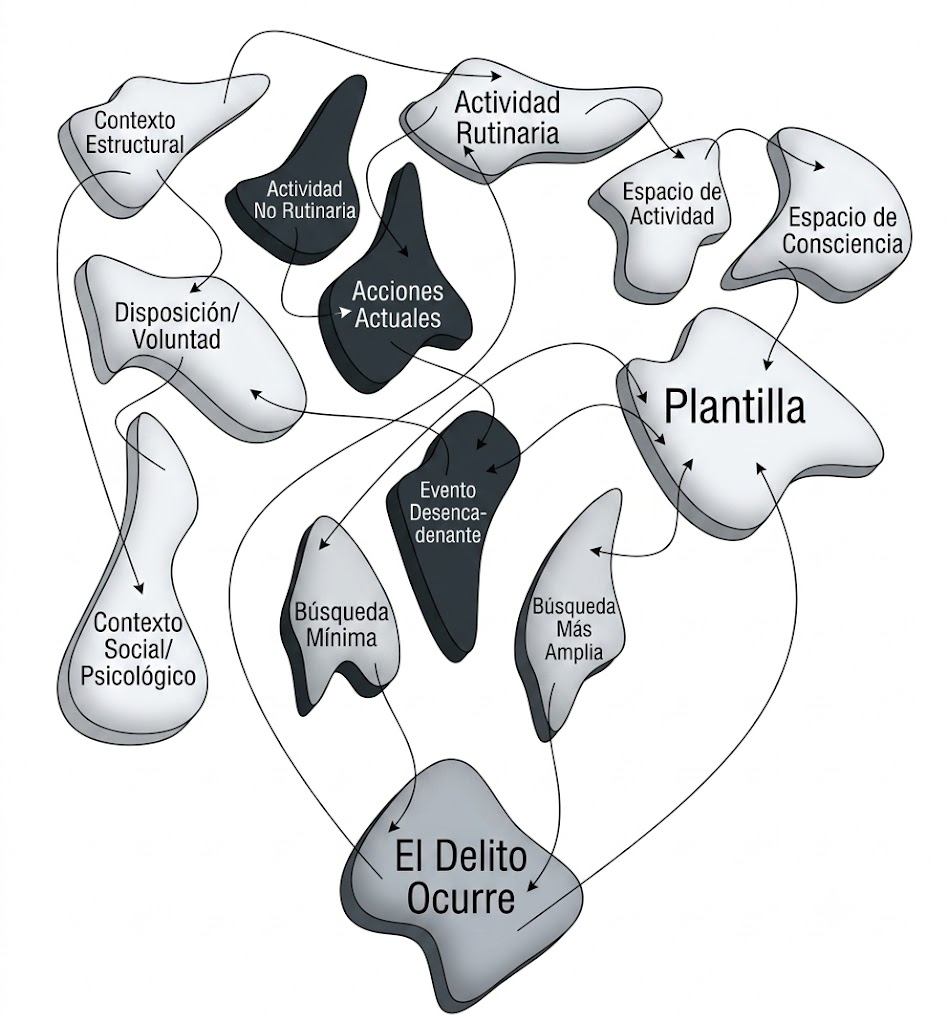
\includegraphics[width=1\linewidth]{figures/capitulo3_marco_teorico/3.1_criminologia_ambiental/teoria_patrones_delictivos_mejorada.png}
    \caption{Procesos, actividades y motivaciones de un crimen}
    \label{fig:patrones_brantingham1993_mejorada}
    \footnotesize{Nota: Adaptación y traducción propia con base en la Figura 11.3 de \cite[p.~284]{brantingham1993}.}
\end{figure}


% =========================================================
% MODELADO DEL TERRENO DE RIESGO (RTM)
% =========================================================
\subsection{Modelado del terreno de riesgo}
El modelado del terreno de riesgo o Risk Terrain Modeling (RTM) es un plan de acción sistemático para estudiar la vulnerabilidad espacial ante el delito\cite{caplan2016}. Identifica los riesgos espaciales que se derivan de las características del paisaje urbano y modela cómo estas se co-localizan para crear entornos únicos para la ocurrencia de delitos específicos\cite{caplan2015}. De esta manera, se busca que factores de riesgo antes tratados como fijos o universales puedan adaptarse a una zona específica con base en su contexto particular y, sobre todo, en los datos disponibles.

El modelo surge como una guía para personas con habilidades básicas en sistemas de información geográfica. Sin embargo, ambos autores desarrollaron a su vez el sistema RTMDx como una implementación técnica que automatiza la mayoría de los pasos analíticos propuestos por el modelo (especialmente los pasos 7 a 9). Así, el proceso actual de RTM y los pasos empleados por el sistema RTMDx son los siguientes\cite[p.~12]{caplan2016}:

\begin{enumerate}
    \item Elegir el evento de resultado
    \item Elegir el área de estudio
    \item Elegir el periodo de tiempo
    \item Identificar los mejores factores de riesgo disponibles
    \item Obtener datos espaciales
    \item Mapear la influencia espacial de los factores
    \item Seleccionar los factores del modelo
    \item Ponderar los factores del modelo
    \item Combinar cuantitativamente los factores del modelo
    \item Comunicar información significativa
\end{enumerate}